\documentclass[12pt,a4paper]{article}

\usepackage{graphicx}% Include figure files
\usepackage{dcolumn}% Align table columns on decimal point
\usepackage{bm}% bold math
%\usepackage{hyperref}% add hypertext capabilities
%\usepackage[mathlines]{lineno}% Enable numbering of text and display math
%\linenumbers\relax % Commence numbering lines

%\usepackage[showframe,%Uncomment any one of the following lines to test 
%%scale=0.7, marginratio={1:1, 2:3}, ignoreall,% default settings
%%text={7in,10in},centering,
%%margin=1.5in,
%%total={6.5in,8.75in}, top=1.2in, left=0.9in, includefoot,
%%height=10in,a5paper,hmargin={3cm,0.8in},
%]{geometry}

\usepackage{multicol}%Para hacer varias columnas
\usepackage{multicol,caption}
\usepackage{multirow}
\usepackage{cancel}
\usepackage{hyperref}
\hypersetup{
    colorlinks=true,
    linkcolor=blue,
    filecolor=magenta,      
    urlcolor=cyan,
}

\setlength{\topmargin}{-1.0in}
\setlength{\oddsidemargin}{-0.3pc}
\setlength{\evensidemargin}{-0.3pc}
\setlength{\textwidth}{6.75in}
\setlength{\textheight}{9.5in}
\setlength{\parskip}{0.5pc}

\usepackage[utf8]{inputenc}
\usepackage{expl3,xparse,xcoffins,titling,kantlipsum}
\usepackage{graphicx}
\usepackage{xcolor} 
\usepackage{nopageno}
\usepackage{lettrine}
\usepackage{caption}
\renewcommand{\figurename}{Figura}
\usepackage{float}
\renewcommand\refname{Bibliograf\'ia}
\usepackage{amssymb}
\usepackage{amsmath}
\usepackage[rightcaption]{sidecap}
\usepackage[spanish]{babel}

\providecommand{\abs}[1]{\lvert#1\rvert}
\providecommand{\norm}[1]{\lVert#1\rVert}
\newcommand{\dbar}{\mathchar'26\mkern-12mu d}

% CABECERA Y PIE DE PÁGINA %%%%%
\usepackage{fancyhdr}
\pagestyle{fancy}
\fancyhf{}

\begin{document}

\textbf{FUNCIONES ESPECIALES}

\begin{enumerate}



%%%1%%%



    \item \textbf{Elabora la monografía correspondiente a las siguientes funciones especiales}
    \begin{enumerate}
        \item \textbf{Polinomios de Laguerre}
        
        
        \item \textbf{Polinomios de Chebychev}
        
        \item \textbf{Polinomios de Legendre}
        
        Ver al final
        \end{enumerate}
    
    
%%%2%%%
    
    
    
    \item \textbf{Un cilindro largo conductor de calor de radio $a$ se compone de dos mitades(con secciones transversales semicirculares) con un espacio infinitesimal entre ellas. Las mitades superior e inferior del cilindro están en contacto con baños térmicos $+T_0$ y $-T_0$, respectivamente. Encuentra la temperatura tanto dentro como fuera del cilindro}
    
    \textbf{SOLUCIÓN:}
    
    \begin{figure}[h!]
        \centering
        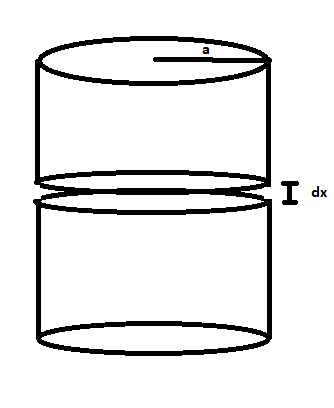
\includegraphics[scale=0.8]{cilindro (2).png}
    \end{figure}
    
    Por la naturaleza del problema, se debe usar la misma ecuación de calor dada por
    
    \begin{equation*}
        u_{t}= \kappa (u_{rr} + \frac{1}{r}u_r + u_{zz}) \hspace{2cm} 0 < r< a \hspace{2cm} t>0 
    \end{equation*}
    
    y también se tienen como condiciones de frontera 
    
    \begin{equation*}
        u(a,z,t)= \left\{ \begin{array}{lcc}
             +T_0 &   si  & z > 0 + \delta z\\
             \\ -T_0 &  si &z < 0 - \delta z\\
             \end{array}
        \right.
    \end{equation*}
    
    con $dz=2\delta z$, con condición inicial $u(a,z,0)=f(r)$
    
    como la distribución de temperatura no depende de $\theta$, podemos proponer como solución a
    
    \begin{equation*}
        u(r,t)= \Omega(r,z)T(t)
    \end{equation*}
    
    y entonces, se tiene que
    
    \begin{equation*}
        u_t= \Omega(r,z)T(t)_t \hspace{0.8cm} u_r=\Omega(r,z)_rT(t) \hspace{0.8cm} u_{rr} = \Omega(r,z)_{rr}T(t) \hspace{0.8cm} u_{zz}= \Omega(r,z)_{zz}T(t)
    \end{equation*}
    
    que sustituyendo
    
    \begin{equation*}
        \Omega(r,z)T(t)_t= \kappa (\Omega(r,z)_{rr}T(t) + \frac{1}{r}\Omega(r,z)_rT(t)+ \Omega(r,z)_{zz}T(t))
    \end{equation*}
    
    dividamos por $\Omega(r,z)T(t)$
    
    \begin{equation*}
        \frac{T(t)_t}{T(t)}= \kappa\left(\frac{\Omega(r,z)_{rr}}{\Omega(r,z)} + \frac{1}{r} \frac{\Omega(r,z)_r}{\Omega(r,z)} + \frac{\Omega(r,z)_{zz}}{\Omega(r,z)}\right)
    \end{equation*}
    
    simplificando la expresión
    
    \begin{equation*}
        \frac{\Omega(r,z)_{rr}}{\Omega(r,z)} + \frac{1}{r} \frac{\Omega(r,z)_r}{\Omega(r,z)} + \frac{\Omega(r,z)_{zz}}{\Omega(r,z)}= \frac{1}{\kappa} \frac{T(t)_t}{T(t)}
    \end{equation*}
    
    al suponer que estas son independientes entre sí, la única forma en la que se cumple la expresión, es 
    
    \begin{equation*}
        \frac{\Omega(r,z)_{rr}}{\Omega(r,z)} + \frac{1}{r} \frac{\Omega(r,z)_r}{\Omega(r,z)} + \frac{\Omega(r,z)_{zz}}{\Omega(r,z)}= \frac{1}{\kappa} \frac{T(t)_t}{T(t)}= - k^2
    \end{equation*}
    
    con $k$ una constante
    

   así, llegamos al sistema de ecuaciones diferenciales ordinarias
   
   \begin{equation*}
       T(t)_t+\kappa k^2T(t)=0
   \end{equation*}
   
   \begin{equation}
       \Omega(r,z)_{rr}+\frac{1}{r}\Omega(r,z)_{r}+\Omega(r,z)_{zz}+k^2 \Omega(r,z)= 0 
   \end{equation}
   
    Ahora, de la ec. (1), propongamos la solución de la forma $\Omega(r,z)=R(r)Z(z)$, y entonces cambiando la notación
    
    \begin{equation*}
        \Omega(r,z)_{rr}= R''(r)Z(z) \hspace{1cm} \Omega(r,z)_r= R'(r)Z(z) \hspace{1cm} \Omega(r,z)_{zz}= R(r)Z''(z)
    \end{equation*}
    
    que sustituyendo en (1)
    
    \begin{equation*}
        R''(r)Z(z)+\frac{1}{r}R'(r)Z(z)+R(r)Z''(z)+ k^2 R(r)Z(z)=0
    \end{equation*}
    
    dividamos por $R(r)Z(z)$
    
    \begin{equation*}
        \frac{R''(r)}{R(r)} + \frac{1}{r} \frac{R'(r)}{R(r)}+\frac{Z''(z)}{Z(z)}+ k^2 =0
    \end{equation*}
    
    dado que cada lado de la igualdad anterior depende de una sola variable, al suponer que estas son independientes entre sí, la única forma en la que se cumple la expresión, es 
    
    \begin{equation*}
        \frac{R''(r)}{R(r)} + \frac{1}{r} \frac{R'(r)}{R(r)}+ k^2=-\frac{Z''(z)}{Z(z)} =-p^2
    \end{equation*}
    
    
    con $p$ contante
   
    y con esto llegamos al sistema de ec. dif, donde $\lambda^2 = k^2+p^2 $
    
    \begin{equation}
        T(t)_t+\kappa k^2T(t)=0
    \end{equation}
    
    \begin{equation}
        R''(r)+ \frac{1}{r} R'(r)+\lambda^2 R(r)=0
    \end{equation}
    
    \begin{equation}
        -Z''(z)+p^2Z(z)=0
    \end{equation}
   
   
   La ec. (3) es una ecuación de tipo Bessel
   
   \begin{equation*}
       y'' + \frac{1}{x}y' + \left(\lambda^2 - \frac{\nu^2}{x^2}\right) y = 0
   \end{equation*}
   
   con $\nu = 0$
   
   Sabemos que la solución general de la ec. dif. de Bessel es de la forma 
   
   \begin{equation*}
       R(r)=C_1J_0(\lambda r)+C_2Y_0(\lambda r)
   \end{equation*}
   
   con $C_1$ y $C_2$ constantes
   
   La función $R(r)$ debe de estar acotada en $r=0$, por lo que se deduce que $C_2 = 0$, ya que $Y_0 (0) \rightarrow \infty$, por lo que
   
   \begin{equation*}
       R(r)=C_1J_0(\lambda r)
   \end{equation*}
   
   y por las condiciones de frontera, tenemos
   
   \begin{equation*}
       \lim_{\delta x \rightarrow 0} Z(z)=\frac{|z|}{z} \hspace{1cm}  \rightarrow \hspace{1cm} p=0
   \end{equation*}
   
   \begin{equation*}
       R(a)T(t)=\frac{|z|}{z} T_0
   \end{equation*}
   
   y como es para todo $t > 0$, entonces
   
   \begin{equation*}
       R(a)=T_0
   \end{equation*}
   
   o bien
   
   \begin{equation*}
       C_1J_0(\lambda a) - T_0 = 0
   \end{equation*}
   
   
   si $\lambda_i$ son las raíces positivas de la ec. anterior, se tiene que aparte del factor constante, las funciones
   
   \begin{equation*}
       R_i(r)=J_0(\lambda_i r)
   \end{equation*}
   
   son soluciones de la ec. (1), para los valores $\lambda$ considerados, la parte temporal tiene las soluciones particulares
   
   \begin{equation*}
       T_i(t)= e^{-\kappa \lambda_{i}^{2} t}
   \end{equation*}
   
   con $\lambda_i > 0$
   
   La suseción de funciones 
   
   \begin{equation*}
       u_i(r,z,t)= \frac{|z|}{z}J_0(\lambda_i t) e^{-\kappa \lambda_{i}^{2}t}
   \end{equation*}
   
   satisfacen la ec. de calor y las condiciones de frontera, y por el principio de superposición
   
   \begin{equation*}
       u(r,z,t)=\frac{|z|}{z} \sum_{i=1}^{\infty}C_i J_0(\lambda_i t) e^{-\kappa \lambda_{i}^{2}t}
   \end{equation*}
   
   tambien satisfacen la ec. de calor y las condiciones de frontera
   
   ahora, ocupando la condición inicial, se obtiene la serie de Fourier-Bessel
   
   \begin{equation*}
       f(r)= \sum_{i=1}^{\infty}C_i J_0(\lambda_i r)
   \end{equation*}
   
   donde 
   
   \begin{equation*}
       C_i = \frac{2}{a^2} \frac{\int_{0}^{a} rf(r)J_0(\lambda_i r) dr}{J_1^2 (\lambda_i a)}
   \end{equation*}
   
   y entonces
   
   \begin{equation*}
       u(r,z,t)=\frac{2|z|}{a^2z} \sum_{i=1}^{\infty}\frac{1}{2J_1^{2}(\lambda_i a)}\left[\int_{0}^{a} rf(r)J_0(\lambda_i r) dr\right] J_0(\lambda_i t) e^{-\kappa \lambda_{i}^{2}t}
   \end{equation*}
   
    
    
    
%%%3%%%
    
    
    
    \item \textbf{Con las propiedades de los polinomios de Hermite, demuestra que:}
    
    \begin{equation*}
        \int_{-\infty}^{\infty} x^2 e^{-x^2} H_n(x)H_n(x)dx = \pi^{\frac{1}{2}} 2^{n} n! (n + \frac{1}{2})
    \end{equation*}
\end{enumerate}

 \textbf{SOLUCIÓN:}
 
 Reescribiendo la relación de recurrencia presentada en las notas de la asesoría 16 en la pagina 21    ($H_{n+1}(x)=2xH_n(x)-2nH_{n-1}(x)$), tenemos
 
 \begin{equation*}
     xH_n(x)= \frac{1}{2}[H_{n+1}(x) + 2nH_{n-1}(x)]
 \end{equation*}
 
 y elevando al cuadrado
 
 \begin{equation*}
   x^2 H_n(x)H_n(x)=\frac{1}{4} [H_{n+1}(x)+2nH_{n-1}(x)]^2
 \end{equation*}
 
 que sustituyendo en la integral
 
 \begin{equation*}
     \int_{-\infty}^{\infty} x^2 e^{-x^2} H_n(x)H_n(x)dx=\frac{1}{4}\int_{-\infty}^{\infty} [H_{n+1}(x)+2nH_{n-1}(x)]^2 e^{-x^2} dx
 \end{equation*}
 
 \begin{equation*}
     =\frac{1}{4}\int_{-\infty}^{\infty}[H_{n+1}(x)H_{n+1}(x) + 2nH_{n+1}(x)H_{n-1}(x)+4n^2H_{n-1}(x)H_{n-1}(x)]e^{-x^2}dx
 \end{equation*}
 
 \begin{equation*}
     =\frac{1}{4}\int_{-\infty}^{\infty}H_{n+1}(x)H_{n+1}(x)e^{-x^2}dx + \frac{n}{2}\int_{-\infty}^{\infty}H_{n+1}(x)H_{n-1}(x)e^{-x^2}dx +n^2\int_{-\infty}^{\infty}H_{n-1}(x)H_{n-1}(x)e^{-x^2}dx
 \end{equation*}

  Ahora por la condición de ortogonalidad presentado en las mismas notas como la ecuación 32 ($\int_{-\infty}^{\infty} e^{-x^2}H_n(x)H_m(x)dx=2^n \sqrt{\pi} n! \delta_{mn}$, donde $\delta_{mn}=0$ si $m\neq n$ y $\delta_{mn}=1$ si $m=n$)
  
  \begin{equation*}
     \int_{-\infty}^{\infty} x^2 e^{-x^2} H_n(x)H_n(x)dx=\frac{1}{4}\int_{-\infty}^{\infty}H_{n+1}(x)H_{n+1}(x)e^{-x^2}dx +n^2\int_{-\infty}^{\infty}H_{n-1}(x)H_{n-1}(x)e^{-x^2}dx
 \end{equation*}
 
 \begin{equation*}
     = \frac{1}{4}(2^{n+1} \sqrt{\pi} (n+1)!)+ n^2(2^{n-1}\sqrt{\pi}(n-1)!)
 \end{equation*}
 
 que reordenando
 
 \begin{equation*}
     \int_{-\infty}^{\infty} x^2 e^{-x^2} H_n(x)H_n(x)dx=\cancel{\frac{4}{4}} (2^{n-1}\sqrt{\pi}(n+1)!)+n^2 (2^{n-1}\sqrt{\pi}(n-1)!)
 \end{equation*}
 
 \begin{equation*}
     = 2^{n-1}\sqrt{\pi}[(n+1)!+n(n-1)!n]
 \end{equation*}
 
 \begin{equation*}
     =2^{n-1}\sqrt{\pi} [n! (n+1)+n! n]
 \end{equation*}
 
 \begin{equation*}
     =2^{n-1}\sqrt{\pi} n! (n+1+n)=2^{n-1}\sqrt{\pi} n! (2n+1) = 2^{n}\sqrt{\pi}n!\left(n+\frac{1}{2}\right)
 \end{equation*}
 
 \begin{equation*}
     \therefore \hspace{1cm} \int_{-\infty}^{\infty} x^2 e^{-x^2} H_n(x)H_n(x)dx=2^{n}\sqrt{\pi}n!\left(n+\frac{1}{2}\right)
 \end{equation*}
 
 $\hspace{15cm} \blacksquare$




\textbf{Problema opcional}

\begin{enumerate}
    \item \textbf{Si se remplaza la condición de que la superficie lateral del cilindro se mantiene a temperatura cero, por la condición de que a través de dicha superficie se transmite calor a una medio circundante que está a temperatura cero, es decir:}
    
    \begin{equation*}
     u_{r}(a,t) =-hu(a,t)  \hspace{2cm} h =cte    
    \end{equation*}
    
    \textbf{Demuestra que la solución es:}
    
    \begin{equation*}
        u(r,t)= \frac{2}{a^2} \sum_{i=1}^{\infty} \frac{\lambda_{i}^{2}}{(\lambda_{i}^{2} + h^2)J_0^2(\lambda_i a)}\left[\int_{0}^{a} rf(r)J_0(\lambda_i r)dr\right] J_0(\lambda_i r) e^{-\kappa \lambda_i^{2}t}
    \end{equation*}
    
    \textbf{Donde la suma es tomada sobre todas las raíces positivas de la ecuación:}
    
    \begin{equation*}
        h J_0(\lambda a)+ \lambda J'_0(\lambda a )=0
    \end{equation*}
    
    
    \textbf{SOLUCIÓN:}
    
    Como solo cambia la condición de frontera del ejercicio resuelto en la asesoría 15, se debe usar la misma ecuación de calor dada por
    
    \begin{equation*}
        u_{t}= \kappa (u_{rr} + \frac{1}{r}u_r) \hspace{2cm} 0 < r< a \hspace{2cm} t>0 
    \end{equation*}
    
    Como la distribución de temperatura no depende de $\theta$ o $z$, podemos proponer como solución a
    
    \begin{equation*}
        u(r,t)= R(r)T(t)
    \end{equation*}
    
    y entonces, se tiene que
    
    \begin{equation*}
        u_t= R(r)T'(t) \hspace{2cm} u_r=R'(r)T(t) \hspace{2cm} u_{rr} = R''(r)T(t)
    \end{equation*}
    
    que sustituyendo
    
    \begin{equation*}
        R(r)T'(t)= \kappa (R''(r)T(t) + \frac{1}{r}R'(r)T(t))
    \end{equation*}
    
    dividamos por $R(r)T(t)$
    
    \begin{equation*}
        \frac{T'(t)}{T(t)}= \kappa\left(\frac{R''(r)}{R(r)} + \frac{1}{r} \frac{R'(r)}{R(r)}\right)
    \end{equation*}
    
    simplificando la expresión
    
    \begin{equation*}
        \frac{R''(r)+ \frac{1}{r} R'(r)}{R(r)}= \frac{1}{\kappa} \frac{T'(t)}{T(t)}
    \end{equation*}
    
    dado que cada lado de la igualdad anterior depende de una sola variable, al suponer que estas son independientes entre ssí, la única forma en la que se cumple la expresión, es 
    
    \begin{equation*}
        \frac{R''(r)+ \frac{1}{r} R'(r)}{R(r)}= \frac{1}{\kappa} \frac{T'(t)}{T(t)}= - \lambda^2
    \end{equation*}
    
    con $\lambda$ una constante, ahora considerando la condición de frontera $u_r(a,t)= -hu(a,t)$
    
    
\begin{equation*}
    R'(a)T(t)=-hR(a)T(t) \rightarrow R'(a)=-hR(a)
\end{equation*}

   así, llegamos al sistema de ecuaciones diferenciales ordinarias
   
   \begin{equation}
       R''(r)+\frac{1}{r}R'(r)+\lambda^2 R(r)= 0 \hspace{2cm} R'(a)=-hR(a)
   \end{equation}
   
   \begin{equation}
       T'(t)+\kappa\lambda^2T(t)=0
   \end{equation}
   
   La ec. (1) es una ecuación de tipo Bessel
   
   \begin{equation*}
       y'' + \frac{1}{x}y' + \left(\lambda^2 - \frac{\nu^2}{x^2}\right) y = 0
   \end{equation*}
   
   con $\nu = 0$
   
   Sabemos que la solución general de la ec. dif. de Bessel es de la forma 
   
   \begin{equation*}
       R(r)=C_1J_0(\lambda r)+C_2Y_0(\lambda r)
   \end{equation*}
   
   con $C_1$ y $C_2$ constantes
   
   La función $R(r)$ debe de estar acotada en $r=0$, por lo que se deduce que $C_2 = 0$, ya que $Y_0 (0) \rightarrow \infty$, por lo que
   
   \begin{equation*}
       R(r)=C_1J_0(\lambda r)
   \end{equation*}
   
   y como $R(a)=-\frac{1}{h}R'(a)$, tenemos
   
   \begin{equation*}
       C_1J_0(\lambda a)= -\frac{1}{h}J'_0(\lambda a)
   \end{equation*}
   
   o bien
   
   \begin{equation*}
       hC_1J_0(\lambda a) = \lambda C_1 J_1(\lambda a)
   \end{equation*}
   
   \begin{equation*}
       hJ_0(\lambda a)- \lambda J_1(\lambda a)=0
   \end{equation*}
   
   si $\lambda_i$ son las raíces positivas de la ec. anterior, se tiene que aparte del factor constante, las funciones
   
   \begin{equation*}
       R_i(r)=J_0(\lambda_i r)
   \end{equation*}
   
   son soluciones de la ec. (1), para los valores $\lambda$ considerados, la parte temporal tiene las soluciones particulares
   
   \begin{equation*}
       T_i(t)= e^{-\kappa \lambda_{i}^{2} t}
   \end{equation*}
   
   con $\lambda_i > 0$
   
   La suseción de funciones 
   
   \begin{equation*}
       u_i(r,t)= J_0(\lambda_i r) e^{-\kappa \lambda_{i}^{2}t}
   \end{equation*}
   
   satisfacen la ec. de calor y las condiciones de frontera, y por el principio de superposición
   
   \begin{equation*}
       u(r,t)= \sum_{i=1}^{\infty}C_i J_0(\lambda_i r) e^{-\kappa \lambda_{i}^{2}t}
   \end{equation*}
   
   tambien satisfacen la ec. de calor y las condiciones de frontera
   
   ahora, ocupando la condición inicial, se obtiene la serie de Fourier-Bessel
   
   \begin{equation*}
       f(r)= \sum_{i=1}^{\infty}C_i J_0(\lambda_i r)
   \end{equation*}
   
   donde 
   
   \begin{equation*}
       C_i = \frac{2}{a^2} \frac{\int_{0}^{a} rf(r)J_0(\lambda_i r) dr}{J_1^2 (\lambda_i a)}
   \end{equation*}
   
   y entonces
   
   \begin{equation*}
       u(r,t)=\frac{2}{a^2} \sum_{i=1}^{\infty}\frac{1}{J_1^{2}(\lambda_i a)}\left[\int_{0}^{a} rf(r)J_0(\lambda_i r) dr\right] J_0(\lambda_i t) e^{-\kappa \lambda_{i}^{2}t}
   \end{equation*}
   
   que por la condición de frontera
  
   
   \begin{equation*}
       u(r,t)=\frac{2}{a^2} \sum_{i=1}^{\infty}\frac{\lambda_i^2}{h^2J_0^{2}(\lambda_i a)}\left[\int_{0}^{a} rf(r)J_0(\lambda_i r) dr\right] J_0(\lambda_i t) e^{-\kappa \lambda_{i}^{2}t}
   \end{equation*}
   
   


\end{enumerate}

\end{document}
